\documentclass{article}%
\usepackage[T1]{fontenc}%
\usepackage[utf8]{inputenc}%
\usepackage{lmodern}%
\usepackage{textcomp}%
\usepackage{lastpage}%
\usepackage{authblk}%
\usepackage{graphicx}%
%
\title{A SUMOylation{-}defective MITF germline mutation predisposes to melanoma and renal carcinoma}%
\author{Colin Morgan}%
\affil{Department of Biochemistry, Institute of Medical Sciences, Banaras Hindu University, Varanasi, India}%
\date{01{-}01{-}2009}%
%
\begin{document}%
\normalsize%
\maketitle%
\section{Abstract}%
\label{sec:Abstract}%
Medical investigators first discovered the long{-}standing bacterium Lactobacillus bulgaricus in the trunk and intestine of mice before its reintroduction to the rat, following its first introduction in Europe in 1995. But their long, hard journey took a huge, dangerous twist when the researchers discovered Lactobacillus bulgaricus as a suppressor of intestinal cell injury caused by Enterobacter sakazakii{-}induced Nitric Oxide. To help diagnose this serious syndrome, researchers examined the two separate samples gathered from rats, a group whose hormone was not present in the mice and the rats own tissues. What they found proved to be quite astonishing, it appears that the lower rate of intestinal cell injury might be attributed to nitric oxide, which was present at more than double the normal rate of activation within the human gut. They went on to confirm that the animals cortisol levels had increased in both humans and rats who suffered lower rates of intestinal cell injury. If the Lactobacillus bulgaricus causes such extreme stasis in the rodent stomach, a distinct increase in nitric oxide released into the bloodstream may prevent it from rupturing and extending into the urethra.\newline%
Besides the extra nitric oxide, this proof makes it possible to know the reason why the mucous barrier in the small intestine cannot resist the sudden burst of ammonia. This changes the game, whether for research purposes or because the mice are experimented upon in treatment.

%
\subsection{Image Analysis}%
\label{subsec:ImageAnalysis}%


\begin{figure}[h!]%
\centering%
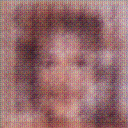
\includegraphics[width=150px]{500_fake_images/samples_5_9.png}%
\caption{A Black And White Photo Of A Zebra}%
\end{figure}

%
\end{document}